% \subsubsection{Model description}
As described in previous papers \sidecite{ogorodnikova_deuterium_2003, hodille_macroscopic_2015, delaporte-mathurin_finite_2019}, the thermokinetics models such as Macroscopic Rate Equation split hydrogen isotopes into two populations: the mobile particles and the trapped ones.
The temporal evolution of mobile particles $c_\mathrm{m}$ and trapped particles $c_{\mathrm{t}, i}$ is described in Equations \ref{eq:mobile} and \ref{eq:trapped} respectively.

\begin{equation}
    \frac{\partial c_\mathrm{m}}{\partial t}=\vec{\nabla} \cdot\left(D(T) \vec{\nabla}c_\mathrm{m}\right)+\Gamma-\sum \frac{\partial c_{\mathrm{t}, i}}{\partial t}
    \label{eq:mobile}
\end{equation}

\begin{equation}
    \frac{\partial c_{\mathrm{t}, i}}{\partial t}=k(T) \cdot c_\mathrm{m} \cdot\left(n_{i}-c_{\mathrm{t}, i}\right)-p(T) \cdot c_{\mathrm{t}, i}
    \label{eq:trapped}
\end{equation}

In Equation \ref{eq:mobile}, ${D(T)=D_0 \exp\big(\frac{-E_\mathrm{D}}{k_B \cdot T}\big)}$ is the diffusion coefficient in \si{m^2.s^{-1}}, $T$ being the temperature in $\si{K}$ and ${k_B = 8.617 \times 10^{-5} \si{eV.K^{-1}}}$ the Boltzmann constant, $\Gamma$ is the volumetric source term of particles in \si{m^{-3}.s^{-1}}, $k(T)=k_0\exp{\big(\frac{-E_{k, i}}{k_B \cdot T}\big)}$ and $p(T)=p_0\exp{\big(\frac{-E_{p, i}}{k_B \cdot T}\big)}$ are the trapping and detrapping rates expressed in \si{m^3.s^{-1}} and \si{s^{-1}} respectively and $n_i$ is the trap density in \si{m^{-3}}.

A more complete description of this model is given in \sidecite{delaporte-mathurin_finite_2019}.
These equations are then solved in FESTIM using the Finite Element Method implemented in FEniCS \sidecite{alnaes_fenics_2015}.
FESTIM is written in Python and provides a user-friendly interface for performing multiphysics, multidimensional and multi-material simulations.

% \subsubsection{Parametric optimisation}
Fitting experimental data by manually tweaking parameters as in \sidecite{yu_deuterium_2019, hodille_macroscopic_2015} can be really time-consuming, sometimes days in some cases.
Moreover, some possible solutions in the parameter space might be missed by the user.
The goal of this study is to automate the parametric optimisation process by embedding FESTIM in a minimisation algorithm.

As in manual fitting, the parametric optimisation problem is solved by minimising a function representing the residual between simulated results and some reference data.
This function $f$ is called \textit{cost function}.
Considering fitting one or several TPD spectra (in order to identify for instance trapping parameters or diffusion coefficients), $f$ can simply be the mean absolute error described in Equation \ref{eq:cost function} representing the residual between the simulated spectrum and the experimental reference: 

\begin{equation}
    f(\textbf{x})=\frac{\sum_{i=0}^{N}  \alpha_i(T_i)\left| d_{i}-d_{\mathrm{sim}}\right|}{\sum_{i=0}^{N}  \alpha_i(T_i)}
    \label{eq:cost function}
\end{equation}

where \textbf{x} is the set of parameters used for the simulation, $d_\mathrm{sim}$ are the values of the simulated spectrum, $N$ is the number of experimental points $(T_i, d_i)$.
In Equation \ref{eq:cost function}, $f(\textbf{x})$ can be weighted by coefficients $\alpha_i$ in order to have a better fit on specific regions of the spectrum.
%Note that this cost function could as well be a root mean square error or any type of residual.

The parametric optimisation problem can now be solved by finding the minimum of the cost function $f$.
The global optimisation routine is illustrated on Figure \ref{fig:diagramm}.
\begin{figure}
    \centering
    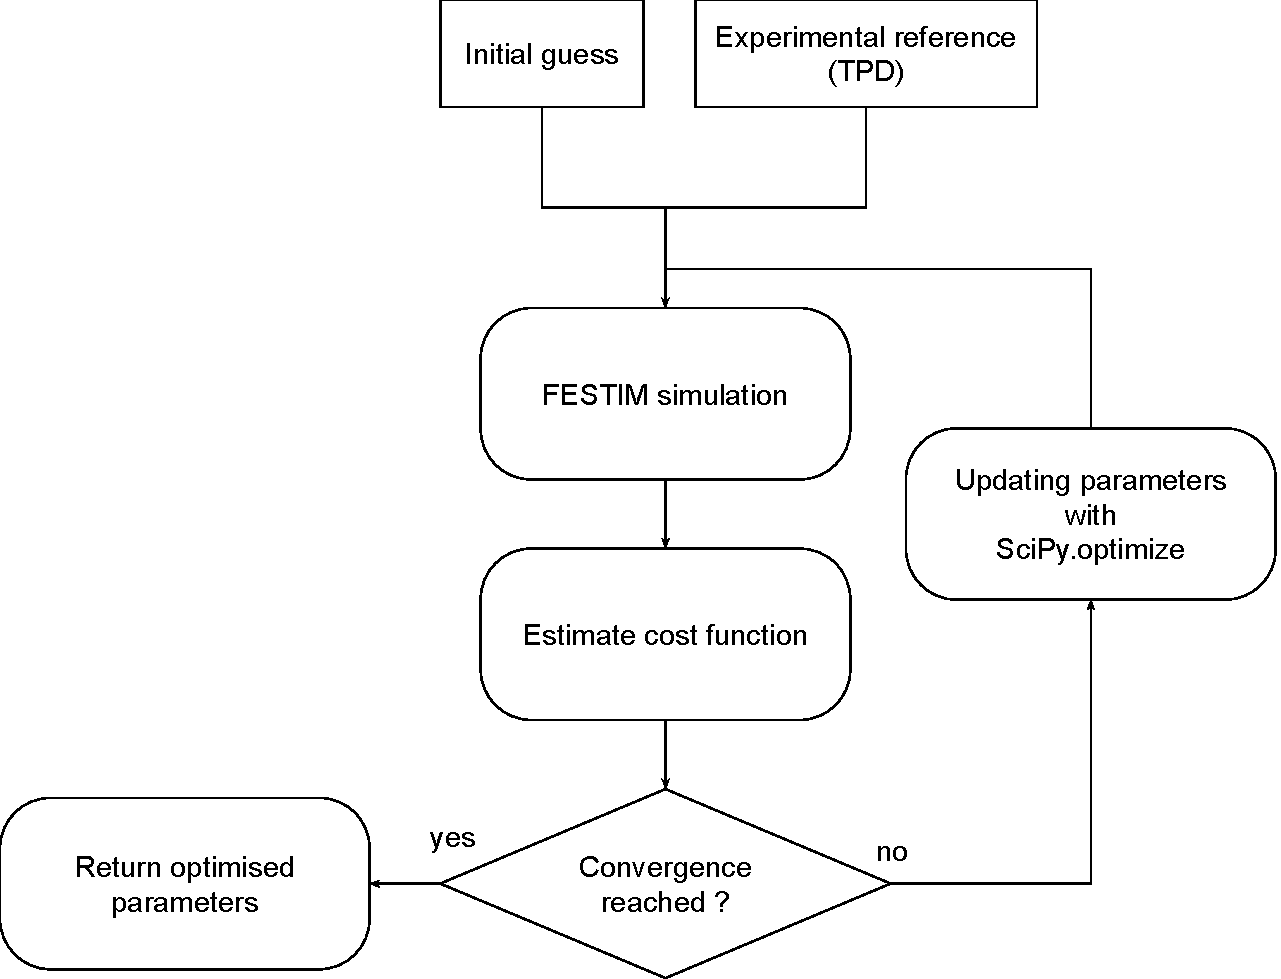
\includegraphics[width=\linewidth]{Figures/Chapter3/Parametric_optimisation/algorithm diagram.pdf}
    \caption{Diagram of the embedding of FESTIM within a parametric optimisation routine based on SciPy \cite{virtanen_scipy_2020}}
    \label{fig:diagramm}
\end{figure}

A comparative study of the several optimisation algorithms which can be employed is made in Section \ref{optimisation algorithms}.
These algorithms require the user to give an initial set of parameters called \textit{initial guess} and evaluate the cost function with several parameters sets until the convergence criterion is reached.
As in \sidecite{drexler_model-based_2019}, the Python package SciPy \sidecite{virtanen_scipy_2020} will be employed.

% \subsubsection{Optimisation algorithms} \label{optimisation algorithms}
In this Section, four minimisation algorithms are benchmarked against a test case.
In the following example an experimental TPD spectrum from Ogorodnikova \textit{et al.} \sidecite{ogorodnikova_deuterium_2003} will be fitted and materials properties such as trap density and detrapping energy will be identified.
For this example case, two intrinsic traps and one extrinsic trap are set.
The only free parameters are $E_1$ and $n_1$, respectively the detrapping energy and density of trap 1.
The other parameters are constrained and described in \sidecite{delaporte-mathurin_finite_2019}.
The cost function $f$ has been plotted on Figure \ref{fig:cost function} as function of $E_1$ and $n_1$.

\begin{figure*} [ht]
    \centering
        \begin{subfigure}[t]{0.5\linewidth}
            \centering
            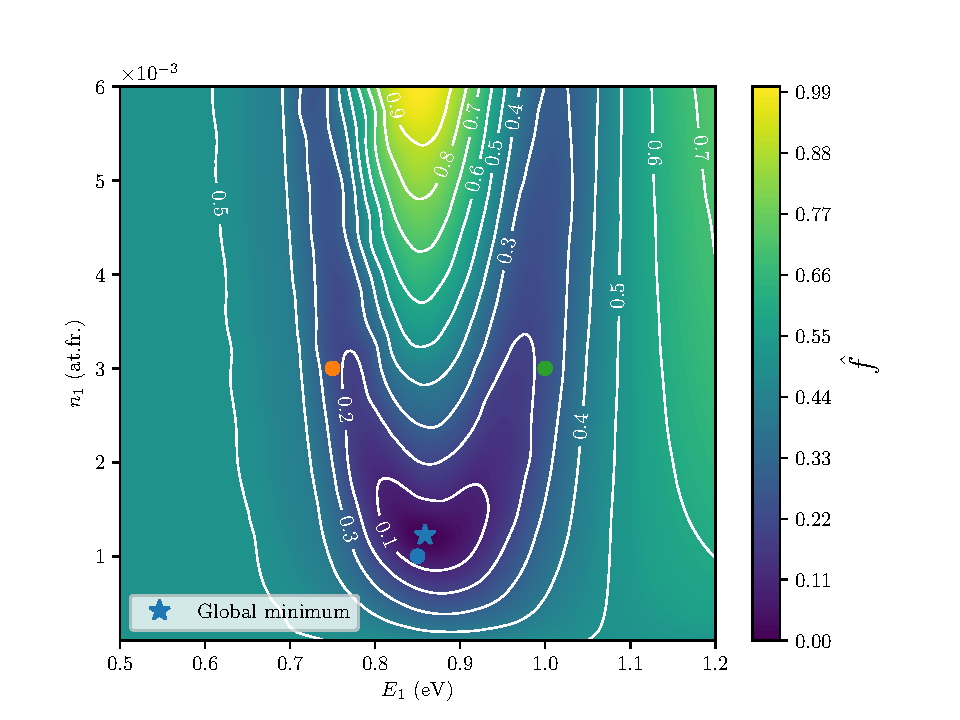
\includegraphics[width=\linewidth]{Figures/Chapter3/Parametric_optimisation/cost_function_2D.pdf}
            \caption{Normalised cost function}
            \label{fig:2D}
        \end{subfigure}%
        \begin{subfigure}[t]{0.5\linewidth}
            \centering
            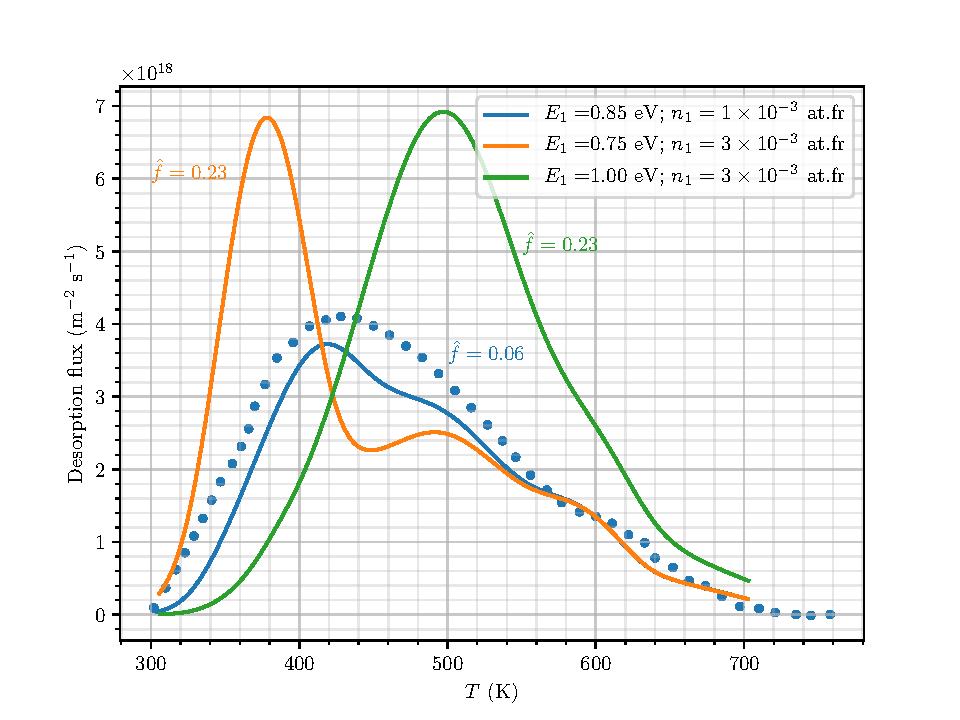
\includegraphics[width=\linewidth]{Figures/Chapter3/Parametric_optimisation/points_on_cost_function.pdf}
            \caption{Corresponding simulated TPD spectra}
            \label{fig:corresponding spectra}
        \end{subfigure}%
    \caption{Normalised cost function $\hat{f} = (f - \min{f})/(\max{f}-\min{f})$ as function of $E_1$ (\si{eV}) and $n_1$ (\si{at.fr.}) with global minimum located at $(\SI{0.86}{eV}, \SI{1.2e-3}{at.fr.})$.}
    \label{fig:cost function}
\end{figure*}

In this case, when only 2 free parameters are set the cost function has only one minimum (it is not necessarily the case for higher dimension optimisation problems).
However, if one fixes the trap density $n_1$ above $\approx \SI{2e-3}{at.fr.}$, the cost function has two local minima which can lead the optimisation routine to converged to a non-global minimum.
Moreover, $f$ is smooth and quadratic around its minimum located at $(E_1, n_1) = (\SI{0.86}{eV}, \SI{1.2e-3}{at.fr.})$.
For detrapping energies below \SI{0.6}{eV} and/or densities below \SI{0.5e-3}{at.fr}, the cost function is constant.
This is because for these values, the contribution of this trapping site to the TPD spectrum is zero either because the density is close to zero, or because the energy is too low for these traps to be filled at the implantation temperature of \SI{300}{K}.
Variations in these regions do not modify the simulated spectrum and thus do not modify the cost function value.

\begin{figure} [ht]
    \centering
    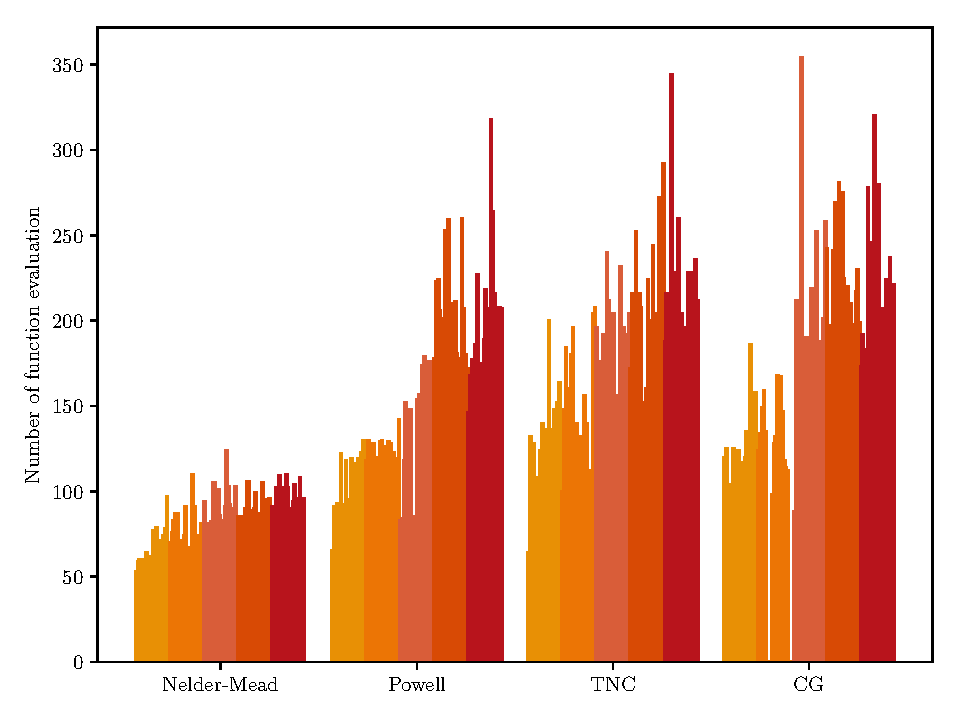
\includegraphics[width=\linewidth]{Figures/Chapter3/Parametric_optimisation/algorithms_perfs.pdf}
    \caption{Number of cost function evaluations required to converge towards the global minimum with 100 different initial guesses sorted by distance to the global minimum for several minimisation algorithms. Each cost function evaluation takes \SI{20}{s} to compute. White stripes correspond to initial guesses for which the algorithm did not converge to the global minimum.}
    \label{fig:algos perfs}
\end{figure}


Four different optimisation algorithms are being compared: 
Nelder-Mead (also called the simplex method), Powell, Truncated Newton method (TNC) and Conjugate Gradient (CG).
Thorough descriptions of these algorithms would be beyond the scope of this study but can be found in \sidecite{nocedal_numerical_2006}.
The performances of these algorithms have been compared with 100 different initial guesses randomly distributed on the $(E_1,n_1)$ plane and are shown on Figure \ref{fig:algos perfs}.
It appears that the CG algorithm is less robust since for some cases it didn't converge towards the global minimum (see white bands on Figure \ref{fig:algos perfs}).
Nelder-Mead algorithm appears to be the most efficient with initial guesses both close and far from the global minimum since the number of cost function evaluations ranges from 50 to 100 whereas other algorithms require more than 100.
This can be explained by the fact that Nelder-Mead is a derivative-free algorithm whereas TNC (Truncated Newton method) and CG algorithms need on the other hand to compute first order derivatives thus increasing the number of function evaluations.
This will be even more true when increasing the number of free parameters since the derivative will become more costly to compute.

It is worth noting that the Nelder-Mead algorithm is an unconstrained method.
If constraints or bounds are needed, TNC might be a more suitable choice.

Though in the following, the Nelder-Mead algorithm will be employed.
